\chapter{Gručenje in razlaga gruč}

Začnimo s primerom. Imam podatke o večini držav sveta, njih skoraj 200, ki jih popišemo s socioekonomskimi značilkami. Značilk imamo, recimo, veliko, vsaj nekaj deset. Vzorec takih podatkov je na primer v tabeli spodaj, a dejansko je naša podatkovna matrika veliko večja.

\begin{table}[htbp]
\caption{Primer profiliranja držav s socioekonomskimi podatki.}
\small
\centering
\renewcommand{\arraystretch}{1.2}
\begin{tabular}{
l
S[table-format=2.1]
S[table-format=2.1]
S[table-format=5.1]
S[table-format=2.1]
S[table-format=2.1]
}
\toprule
\makecell[l]{Država} &
{\makecell[b]{Pričakovana \\ življenjska \\ doba}} &
{\makecell[b]{Povprečno \\ število let \\ šolanja}} &
{\makecell[b]{BDP na \\ prebivalca}} &
{\makecell[b]{Delež \\ urbanega \\ prebivalstva}} &
{\makecell[b]{Necepljeni \\ dojenčki \\ (ošpice)}} \\
\midrule
Avstralija & 82.5 & 13.2 & 42822.0 & 89.4 & 7.0 \\
Čile       & 82.0 & 9.9  & 21665.0 & 89.5 & 6.0 \\
Kuba       & 79.6 & 11.8 & 7455.0  & 77.1 & 1.0 \\
Danska     & 80.4 & 12.7 & 44519.0 & 87.7 & 10.0 \\
Grčija     & 81.1 & 10.5 & 24808.0 & 78.0 & 3.0 \\
Slovenija  & 80.6 & 12.1 & 28664.0 & 49.7 & 6.0 \\
Švica      & 83.1 & 13.4 & 56364.0 & 73.9 & 7.0 \\
Venezuela  & 74.4 & 9.4  & 15129.0 & 89.0 & 11.0 \\
\bottomrule
\end{tabular}
\label{tab:podatki-drzave}
\end{table}

Nad takimi podatki lahko izvedemo gručenje, torej postopek, kjer podatke razdelimo v skupine (gruče) glede na njihovo podobnost. V tem poglavju bomo postopke gručenja skušali predstaviti sistematično, a šele kasneje, saj jih je, prvič, bralec skozi svoje dosedanje šolanje najbrž že spoznal, in drugič, ker se bomo najprej posvetili postopkom razlage gruč. Tretjič pa zato, ker smo nekatere postopke za iskanje gruč že spoznali v prejšnjem poglavju, ko smo gradili podatkovne karte oziroma smo podatke skušali predstaviti v dvorazsežnem razsevnem diagramu. Primer takšne podatkovne karte je prikazan na sliki~\ref{fig:tsne-izbor}.

\begin{marginfigure}
    \centering
    \includegraphics[width=0.8\linewidth]{figs/070-tsne-izbor.pdf}
    \caption{Države v grafu t-SNE. Za gradnjo grafa smo uporabili podatkovni nabor {\em Human Development Index} iz leta 2014 z 50 značilkami. Med državami na grafu smo izbrali manjšo skupino.}
    \label{fig:tsne-izbor}
\end{marginfigure}

Na podatkovni karti s slike~\ref{fig:tsne-izbor} lahko razberemo nekaj skupin. Izbrali smo eno izmed njih, z osmimi državami, in želimo vedeti, kaj je tem državam skupnega. Imamo nekaj možnosti:
\begin{itemize}
\item Imena držav lahko izpišemo. To bo za osem držav najbrž prva stvar, ki jo lahko naredimo, problem pa bi bil, če bi bila izbrana skupina večja in manj pregledna.
\item Pogledamo, kje so te države na zemljevidu. Zemljevid nam ponuja dodatno informacijo, ki sicer ni vsebovana v podatkih, a nam pride prav, sploh če nam geografija ni tuja.
\item Lahko si pomagamo s podatki o skupinah držav, na primer mediteranske, azijske, južnoameriške, in potem ugotovimo, ali večina držav, ki smo jih izbrali, pripada kakšni od teh skupin.
\item Razmišljamo lahko, v katerih značilnostih so izbrane države različne od vseh ostalih. Še najbolj prav bi nam tu prišel urejen seznam atributov, od atributov, kjer se izbrane države najbolj ločijo od vseh ostalih, do atributov, kjer je ta ločitev slabša ali pa je ni. Seveda nam bodo tu pomagala socioekonomska znanja za razumevanje tega urejenega seznama.
\item Če imamo atributov veliko, bi nam lahko pomagala ureditev atributov v skupine. Recimo, določili bi lahko atribute, ki so povezani z zdravstvom, pa s finančnimi kazalci, šolstvom in podobnim. Potem bi morda lahko za izbrane države ugotovili, da so to med najpremožnejšimi državami na svetu ali pa med državami z najbolj razvitim šolstvom in podobno.
\end{itemize}

Zgoraj našteti so različni načini razlage skupin. Pri nekaterih smo uporabili vedenje o (izbranih) primerih, pri drugih pa smo skušali izbrane primere (diferencialno) opisati z uporabo podatkov. Pri večini nekoliko boljših razlag nam je prav prišlo neko dodatno znanje oziroma informacije, ki niso bile prisotne v sami tabeli podatkov. Takemu znanju pravimo tudi domensko znanje. Pri vseh zgornjih idejah, razen morda pri prvih dveh, bomo sicer morali uporabiti neke računske postopke za rangiranje atributov ali pa ugotavljanje obogatenosti skupin. In prav o teh bo govor v nadaljevanju besedila.

\section{Analiza obogatenosti skupin}

Poenostavimo zgornji primer in predpostavimo, da smo v podatkih imeli samo 12 držav in med njimi našli skupino petih, kot to kaže tabela~\ref{tab:drzave-izbor}. Opazimo, da je med izbranimi državami kar nekaj mediteranskih.
%
\marginnote{Pojavu, da se neka skupina v izboru pojavlja pogosteje, kot bi pričakovali pri naključnem izboru iz celotne množice, pravimo obogatenost skupine.}
%
Pravzaprav je v tabeli pet mediteranskih držav (Francija, Grčija, Hrvaška, Italija, Španija), med njimi pa so kar štiri države iz našega izbora. V našem izboru je tudi Portugalska, ki ni mediteranska država. Vprašamo se, ali bi tako veliko (ali večje) število mediteranskih držav v našem izboru dobili tudi po naključju. Torej, kakšna je verjetnost, da bi pri naključnem izboru petih držav izmed vseh dvanajstih izbrali vsaj štiri mediteranske države?

Pomagajmo si s kombinatoriko. Naši podatki vsebujejo končno množico $N=12$ držav, med katerimi je $K=5$ mediteranskih držav. Iz te množice smo izbrali $n=5$ držav, pri čemer je bilo $k=4$ mediteranskih. Verjetnost, da v izboru dobimo natanko \(k\) mediteranskih držav, je enaka
\[
P(X=k)=\frac{\binom{K}{k}\binom{N-K}{n-k}}{\binom{N}{n}}.
\]
Ta izraz je znan kot hipergeometrična porazdelitev, ki opisuje verjetnosti pri vzorčenju brez vračanja iz končne množice. V našem primeru slučajna spremenljivka \(X\), ki šteje število mediteranskih držav v izboru, sledi hipergeometrični porazdelitvi s parametri \(N\), \(K\) in \(n\).

\begin{margintable}
\caption{Države in njihov izbor. Izbrane države so označene v koloni ``Izbor'' z 1, ostale z 0.}
\vspace{2mm}
\begin{tabular}{lc}
\toprule
Država & Izbor \\
\midrule
Avstrija     & 0 \\
Francija     & 1 \\
Grčija       & 1 \\
Hrvaška      & 0 \\
Italija      & 1 \\
Nemčija      & 0 \\
Nizozemska   & 0 \\
Portugalska  & 1 \\
Poljska      & 0 \\
Španija      & 1 \\
Švedska      & 0 \\
Švica        & 0 \\
\bottomrule
\end{tabular}
\label{tab:drzave-izbor}
\end{margintable}

V hipergeometrični porazdelitvi je \(\binom{K}{k}\) število načinov, kako izmed vseh \(K\) mediteranskih držav izberemo \(k\) držav, \(\binom{N-K}{n-k}\) število načinov, kako izmed vseh nemediteranskih držav izberemo preostalih \(n-k\) držav, \(\binom{N}{n}\) pa število vseh možnih izborov \(n\) držav iz celotne množice \(N\) držav. Ulomek tako predstavlja delež vseh možnih izborov, v katerih je natanko \(k\) mediteranskih držav.

V našem primeru smo opazili \(X=4\), saj so med petimi izbranimi državami štiri mediteranske. Ker nas zanima, ali je to nenavadno velik delež, računamo verjetnost, da bi po naključju dobili vsaj štiri mediteranske države:
\[
P(X\ge 4)=P(X=4)+P(X=5).
\]

Dobimo
\[
P(X=4)=\frac{\binom{5}{4}\binom{7}{1}}{\binom{12}{5}}
=\frac{5\cdot 7}{792}
=\frac{35}{792},
\]
in
\[
P(X=5)=\frac{\binom{5}{5}\binom{7}{0}}{\binom{12}{5}}
=\frac{1\cdot 1}{792}
=\frac{1}{792}.
\]
Skupaj je torej
\[
P(X\ge 4)=\frac{35}{792}+\frac{1}{792}
=\frac{36}{792}
=\frac{1}{22}
\approx 0{,}0455.
\]

To pomeni, da bi pri povsem naključnem izboru petih držav izmed dvanajstih dobili vsaj štiri mediteranske države z verjetnostjo približno \(4{,}5\%\). Tak rezultat je torej razmeroma malo verjeten in kaže na to, da so mediteranske države v našem izboru obogatene glede na to, kar bi pričakovali po naključju.

Za dodatno orientacijo lahko pogledamo še pričakovano število mediteranskih držav v naključnem izboru petih držav. Za hipergeometrično porazdelitev velja, da je pričakovana vrednost enaka
\[
E(X)=n\frac{K}{N}=5\cdot\frac{5}{12}=\frac{25}{12}\approx 2{,}08.
\]
V naključnem izboru bi torej v povprečju pričakovali nekaj več kot dve mediteranski državi, opazili pa smo kar štiri. Tudi tako vidimo, da je naš rezultat drugačen od pričakovanega pri naključnem izboru.

Seveda bi namesto mediteranske skupine lahko vzeli tudi kakšno drugo skupino držav. Recimo, države evrobmočja. Med dvanajstimi državami v naših podatkih je takih držav devet, med petimi izbranimi državami pa so vse članice evroobmočja. Če označimo z \(X\) število držav evroobmočja v izboru, velja \(N=12\), \(K=9\), \(n=5\) in \(k=5\). Verjetnost, da bi pri naključnem izboru petih držav dobili same države evroobmočja, je
\[
P(X=5)=\frac{\binom{9}{5}\binom{3}{0}}{\binom{12}{5}}
=\frac{126}{792}
\approx 0{,}159.
\]
Tak rezultat torej ni posebno malo verjeten, zato v tem primeru ne bi mogli govoriti o izraziti obogatenosti.

Obogatenost je torej pojav, ko se elementi določene skupine v izboru pojavljajo pogosteje, kot bi pričakovali po naključju. Analiza obogatenosti pa je postopek, s katerim to odstopanje kvantitativno ovrednotimo in preverimo, ali ga lahko pripišemo naključju ali pa kaže na dejanski vzorec v podatkih.

\section{Analiza obogatenosti v kodi}

Z analizo obogatenosti lahko torej razložimo, kateri skupini primerov pripadajo izbrani primeri tako, da je ta pripadnost (močno) drugačne od naključne. Za to poleg podatkov pripravimo domensko znanje v obliki skupin, za naš primer na primer v zapisu, kot je prikazan na sliki~\ref{fig:skupine-drzav}.

\begin{marginfigure}
\caption{Zapis v obliki YAML s primerom določitve skupin držav.}
\label{fig:skupine-drzav}
\footnotesize
\begin{verbatim}
Mediteranske:
  - Francija
  - Grčija
  - Hrvaška
  - Italija
  - Španija

Balkanske:
  - Grčija
  - Hrvaška

Zahodnoevropske:
  - Francija
  - Nemčija
  - Nizozemska
  - Avstrija
  - Švica
\end{verbatim}
\end{marginfigure}

Za izračun obogatenosti bomo uporabili funkcijo \texttt{hypergeom.sf} iz knjižnice \texttt{scipy.stats}, kjer je \texttt{sf} tako imenovana funkcija preživetja (angl. {\em survival function}) in nam vrne verjetnost, da je slučajna spremenljivka $X$ večja od določene vrednosti $k$. 
%
\vspace*{3mm}
\begin{lstlisting}
def enrichment(all_items, selected_items, group):
    group = set(group) & all_items

    N = len(all_items)
    n = len(selected_items)
    K = len(group)
    k = len(group & selected_items)

    p_value = hypergeom.sf(k - 1, N, K, n) if K > 0 else 1.0
    expected = n * K / N if N > 0 else 0.0
    fold = (k / expected) if expected > 0 else float("nan")

    return {
        "K": K,
        "k": k,
        "expected": expected,
        "fold": fold,
        "p_value": p_value,
    }
\end{lstlisting}
%
Vhod v našo funkcijo obogatenosti \texttt{enrichment} 
%
\marginnote{Statistična značilnost opisuje, kako verjetno je, da bi opažen rezultat nastal zgolj zaradi naključja. To ocenimo s $p$-vrednostjo: manjša kot je, manj verjetno je, da je rezultat posledica naključnega izbora.}
%
so množica vseh objektov, množica izbranih objektov in skupina, za katero računamo obogatenost oziroma verjetnost, da bi izbrani objekti pripadali tej skupini, če bi bil izbor naključen. Funkcija vrne parametra porazdelitve $K$ in $k$, pričakovano vrednost (koliko elementov iz dane skupine bi pričakovali med izbranimi objekti pri naključnem izboru) faktor obogatenosti (razmerje dejanske in pričakovane vrednosti), in končno še $p$-vrednost, ki ocenjuje statistično značilnost opaženega prekrivanja.

\begin{marginfigure}
    \centering
    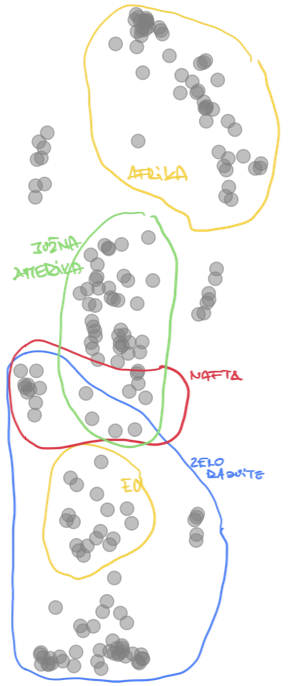
\includegraphics[width=0.8\linewidth]{figs/070-tsne-anotacija.png}
    \caption{Primer možne anotacije t-SNE razporeditve držav v dvodimenzionalno karto. Bi znali tako razlago karte sprogramirati?}
    \label{fig:tsne-anotacija}
\end{marginfigure}


V glavnem delu naše implementacije preberemo podatke o izboru, podatke o skupinah držav, izračunamo obogatenost in izpišemo rezultate:
\vspace*{3mm}
\begin{lstlisting}
import yaml
import pandas as pd

df = pd.read_excel("izbrane-države.xlsx")

all_items = set(df["Država"].astype(str).str.strip())
selected_items = set(
    df.loc[df["Izbor"] == 1, "Država"].astype(str).str.strip()
)

with open("skupine-držav.yaml", "r", encoding="utf-8") as f:
    groups = yaml.safe_load(f)

results = []
for name, group in groups.items():
    r = enrichment(all_items, selected_items, group)
    r["group"] = name
    results.append(r)

results.sort(key=lambda x: x["p_value"])

for r in results:
    print(
        f"{r['group']+":":20s} "
        f"k={r['k']:2d}, K={r['K']:2d}, "
        f"E={r['expected']:.2f}, "
        f"fold={r['fold']:.2f}, "
        f"P={r['p_value']:4f}"
    )
\end{lstlisting}

Analiza obogatenosti za naš izbor držav in skupine držav, s katerimi predstavimo domensko znanje, torej vrne po $p$-vrednosti urejen seznam skupin:
%
{\small
\begin{verbatim}
Mediteranske:        k= 4, K= 5, E=2.08, fold=1.92, P=0.0455
Evroobmočje:         k= 5, K= 9, E=3.75, fold=1.33, P=0.1591
Obmorske:            k= 5, K=10, E=4.17, fold=1.20, P=0.3182
Balkanske:           k= 1, K= 2, E=0.83, fold=1.20, P=0.6818
Zahodnoevropske:     k= 1, K= 5, E=2.08, fold=0.48, P=0.9735
\end{verbatim}
}
%
Pravzaprav nas zanimajo samo skupine, ki so statistično značilne in kjer je njihova naključna verjetnost zelo majhna. Za to pa rabimo določiti prag, 
%
\marginnote{Parameter $\alpha$ določa verjetnost napake tipa I, torej da napačno razglasimo rezultat za statistično značilen, čeprav je v resnici posledica naključja.}
%
običajno označen z $\alpha$ (npr. $\alpha = 0{,}05$), pod katerim $p$-vrednost štejemo kot dovolj majhno. Skupine z $p < \alpha$ tako obravnavamo kot obogatene, ostale pa kot posledico naključnega izbora.

Kako se potem lotim razlage morebitnih skupin s slike~\ref{fig:tsne-izbor}? Lahko z izdelavo interaktivne vizualizacije, kjer bi uporabniku omogočili izbor točk oziroma držav iz vizualizacije in potem prikazali obogatene skupine. Še boljša pa bi bila avtomatična prepoznava gruč točk na vizualizaciji in potem anotacija teh gruč z imeni obogatenih skupin. Nekaj podobnega (sicer izmišljeni) razlagi s slike~\ref{fig:tsne-anotacija}.

\begin{exercise}{Preveč skupin, premalo statistike.}
  Ustvari $100$ primerov in jih naključno razdeli v dve skupini po $50$; eno skupino obravnavaj kot izbor (\texttt{selected\_items}), drugo kot preostanek. Nato generiraj $m$ naključnih skupin (vsaka je naključna podmnožica vseh primerov) in za vsako izračunaj obogatenost z \texttt{enrichment}. Preštej, koliko skupin ima $p<0{,}05$. Ponovi za $m=100$ in $m=1000$ (z istim izborom ali z več ponovitvami). Kaj se zgodi s številom obogatenih skupin, ko povečuješ $m$?
\end{exercise}  

\section{Večkratno testiranje}

V zgornjem primeru smo testirali le nekaj skupin držav. Število skupin pa je pogosto precej večje. Države iz našega primera bi lahko bile na primer označene z mnogimi geografskimi, političnimi, gospodarskimi, kulturnimi in zgodovinskimi oznakami. Če je teh testiranih skupin veliko, se lahko zgodi, da so nekatere skupine videti statistično značilne zgolj po naključju.

Gre za {\em problem večkratnega testiranja} (angl. {\em multiple testing problem}): če izvedemo veliko ločenih testov, bodo nekateri rezultati videti statistično značilni že zaradi naklučja. Predpostavimo, da testiramo 100 skupin in uporabimo prag $\alpha = 0.05$. Tudi če nobena skupina v resnici ni obogatena, bi s to izbiro $\alpha$ zaradi naključja pričakovali približno pet skupin značilno obogatenih skupin ($p < 0.05$). Zato so lahko pri velikem številu testov izvedene vrednosti $p$ zavajajoče.

Ena najbolj znanih popravkov je te meje je Bonferronijev popravek.
%
\marginnote{Bonferronijev popravek je poimenovan po Carlu Emiliu
Bonferroniju, njegova osnova pa izhaja iz njegovega dela o verjetnostnih
neenakostih iz leta 1936.}
%
Po njem, ko izvedemo $m$ testov, prag $\alpha$ nadomestimo z
\[
\alpha' = \frac{\alpha}{m}.
\]
Bonferronijev popravek je zelo konservativen: močno zmanjša verjetnost lažnih odkritij, vendar lahko hkrati prikrije tudi nekatere dejansko obogatene skupine.

Manj konservativen in pogosto uporabnejši pristop je nadzorovanje {\em stopnje lažnih odkritij} ({\em false discovery rate}, FDR).
%
\marginnote{Stopnjo lažnih odkritij (FDR) sta leta 1995 uvedla Yoav Benjamini in Yosef Hochberg v članku ``Controlling the False Discovery Rate: A Practical and Powerful Approach to Multiple Testing'' v reviji {em Journal of the Royal Statistical Society: Series B}.}
%
FDR predstavlja pričakovani delež lažnih odkritij med vsemi rezultati, ki jih razglasimo za statistično značilne. Če na primer nadzorujemo FDR na ravni $\alpha = 0.05$, sprejmemo možnost, da je med skupinami, ki jih razglasimo za obogatene, približno $5\,\%$ lažnih odkritij. Popravek lahko razumemo kot način prilagajanja vrednosti $p$. Najprej vseh $m$ vrednosti $p$ uredimo od najmanjše do največje:
\[
p_{(1)} \le p_{(2)} \le \cdots \le p_{(m)}.
\]
Vsako urejeno vrednost $p$ nato pomnožimo s faktorjem, ki je odvisen od
njenega ranga:
\[
p_{(i)}^\ast = p_{(i)}\frac{m}{i}.
\]
Tako najmanjšo vrednost $p$ pomnožimo z $m$, drugo najmanjšo z $m/2$, tretjo z $m/3$ in tako naprej. Nato prilagojene vrednosti dodatno popravimo, da so monotono naraščajoče in se pri prehodu od manjših proti večjim izvirnim vrednostim $p$ ne zmanjšujejo. Tako dobljene prilagojene vrednosti $p$ lahko primerjamo z običajnim pragom $\alpha$. Skupine, katerih prilagojena vrednost $p$ je manjša od $\alpha$, označimo kot statistično značilne.

V primerjavi z Bonferronijevim popravkom je Benjamini--Hochbergov popravek običajno manj strog, zato pogosto odkrije več obogatenih skupin, hkrati pa še vedno omejuje pričakovani delež lažnih odkritij med prijavljenimi rezultati.

V praksi bi morala analiza obogatitve zato poročati ne le o surovih vrednostih $p$, temveč tudi o popravljenih vrednostih $p$ oziroma o oceni FDR, zlasti kadar testiramo veliko število skupin. Pri majhnem številu skupin popravek morda ne bo bistveno spremenil sklepov. Pri tisočih testiranih skupinah pa lahko popolnoma spremeni, katerim razlagam lahko zaupamo.

\section{S skupinami povezane zvezne značilke}

Vrnimo se k našemu izboru skupine držav s slike~\ref{fig:tsne-izbor}, a se tokrat osredotočimo na njihove lastnosti. Radi bi ugotovili, v katerih značilkah se izbrana skupina razlikuje od vseh drugih. V podatkih, iz katerih smo zgradili vizualizacijo, je bilo 50 značilk, zato bi bilo smiselno dobiti urejen seznam, kjer so na vrhu tiste, ki so z našim izborom najbolj povezane. Potrebujemo torej neko cenilko povezanosti skupine z informativnostjo značilke, ki zavzame večje vrednosti za značilke, pri katerih se izbrane države najbolj razlikujejo od preostalih.

Začnimo sicer s hipotetičnim primerom in za tri značilke, imenovali smo jih kar $A$, $B$, in $C$, prikažimo, kakšna je njihova porazdelitev vrednosti v izbrani množici držav in kako so te vrednosti porazdeljene v vseh ostalih državah (slika~\ref{fig:porazdelitve}). Katera značilka je najbolj informativna? Katera torej najbolje loči primere iz izbrane gruče od vseh ostalih primerov? Porazdelitvi sta ločeni pri značilkah $A$ in $B$, a je prekrivanje pri značilki $B$ manjše. Prekrivanje je veliko pri značilki $C$. 

Očitno nam o izbrani skupini
%
\marginnote{Statistiko $t$ je uvedel William Sealy Gosset leta 1908.
Objavil jo je pod psevdonimom Student v članku ``The probable error of a mean'', saj je delal za pivovarno Guinness, ki svojim zaposlenim ni dovoljevala objavljanja znanstvenih del pod lastnim imenom. Zato danes govorimo o Studentovi t-porazdelitvi in t-testu.}
%
največ informacij poda značilka $B$. Intuitivno lahko rečemo, da so boljše tiste značilke, pri katerih sta porazdelitvi čim bolj odmaknjeni druga od druge in hkrati čim manj razpršeni. Odmaknjenost lahko ocenimo z razliko med povprečnima vrednostma obeh skupin, razpršenost pa z varianco. Ker želimo eno samo cenilko, ki upošteva oboje, lahko uporabimo $t$-statistiko. Ta meri razliko med povprečjema glede na razpršenost podatkov v obeh skupinah. Za značilko $X$ jo zapišemo kot
\[
t = \frac{\bar{x}_1 - \bar{x}_2}{\sqrt{\frac{s_1^2}{n_1} + \frac{s_2^2}{n_2}}},
\]
kjer sta $\bar{x}_1$ in $\bar{x}_2$ povprečji v izbrani in preostali skupini, $s_1^2$ in $s_2^2$ varianci, $n_1$ in $n_2$ pa velikosti obeh skupin. Večja absolutna vrednost $t$ pomeni večjo ločljivost med skupinama in s tem večjo informativnost značilke.

\begin{marginfigure}
    \caption{Porazdelitev spremenljivk $A$, $B$ in $C$ v izbrani skupini primerov (oranžna) in v vseh ostalih primerih (modra).}
    \centering
    \includegraphics[width=0.7\linewidth]{figs/070-porazdelitve.pdf}
    \label{fig:porazdelitve}
\end{marginfigure}

Za rangiranje značilk bo absolutna vrednost $t$ dovolj, če pa želimo oceniti tudi statistično značilnost opažene razlike, $t$ pretvorimo v $p$-vrednost. To dobimo iz $t$-porazdelitve kot verjetnost, da bi ob predpostavki, da razlike med skupinama ni, dobili tako veliko ali še večjo vrednost $|t|$. Pri tem predpostavimo, da $t$ sledi $t$-porazdelitvi z ustreznim številom prostostnih stopenj (npr. $\nu \approx n_1 + n_2 - 2$) in izračunamo repno verjetnost. Za dvostranski test velja
\[
p = 2 \cdot P(T \ge |t|).
\]
Manjša kot je $p$-vrednost, manj verjetno je, da je opažena razlika posledica naključja. V Pythonu to izračunamo kot:

\vspace*{3mm}
\begin{lstlisting}
from scipy.stats import t
p_value = 2 * t.sf(abs(t_stat), df)
\end{lstlisting}

S kodo, ki bi primerno prebrala podatke, nam omogočila izbor neke skupine držav in potem izračunala $t$-statistiko oziroma njeno pripadajočo $p$-vrednost bi lahko dobili izpis, katerega primer je na primer spodaj:
\vspace*{3mm}
\begin{lstlisting}
0.0000 v Neenakost v življenjski dobi (%)
0.0000 v Umrljivost dojenčkov (na 1000 rojstev)
0.0006 v Mladi brez šole in zaposlitve (%)
0.0012 v Dojenčki izključno dojeni (%)
0.0014 v Neenakost v dohodku (%)
0.0294 ^ Delež žensk v parlamentu (%)
0.0769 ^ Plačan porodniški dopust (dni)
\end{lstlisting}
Ta poleg $p$-vrednosti tudi pove, ali je vrednost značilke v izbrani skupini manjša ali večja. Seveda bi bilo zelo primerno, če bi za tako analizo razvili primerni uporabniški vmesnik, ki bi nam na enostaven način omogočil raziskovanje podatkov in njihovih skupin.

\section{Kaj pa, če so spremenljivke kategorične?}

Zgornje predpostavlja, da so vse značilke zvezne. Kaj pa, če so te kategorične (recimo spol, regija ali tip države)? V tem primeru lahko namesto cenilke $t$ uporabimo $\chi^2$-statistiko, ki meri odstopanje med opaženimi in pričakovanimi frekvencami v kontingenčni tabeli.

Predpostavimo, da je med 12 državami 8 članic OECD, 4 pa niso, in da tabela podatkov (glej tabelo~\ref{tab:podatki-drzave}) vsebuje značilko, ki o tem članstvu poroča. Naj bodo v izbrani skupini petih držav, kjer so 4 članice OECD in 1 ni. Ta razmerja lahko predstavimo v kontingenčni tabeli~\ref{tab:oecd}.

\begin{margintable}
\caption{Kontingenčna tabela članstva v OECD.}
\begin{center}
\small
\begin{tabular}{lcc}
\toprule
 & Izbrane & Ostale \\
\midrule
OECD     & 4 & 4 \\
Ne-OECD  & 1 & 3 \\
\midrule
Skupaj   & 5 & 7 \\
\bottomrule
\end{tabular}
\end{center}
\label{tab:oecd}
\end{margintable}

Če članstvo v OECD z izborom ne bi bilo povezano, bi pričakovane frekvence izračunali kot
\[
E_{ij}=\frac{(\text{vsota vrstice})\cdot(\text{vsota stolpca})}{\text{skupna vsota}}.
\]

Tako za članice OECD v izbrani skupini dobimo
\[
E=\frac{8\cdot 5}{12}=3{,}33,
\]
za nečlanice OECD pa
\[
E=\frac{4\cdot 5}{12}=1{,}67.
\]

Odstopanje med opaženimi in pričakovanimi frekvencami bomo kvantitativno izmerili s statistiko \(\chi^2\), ki združuje prispevke vseh celic kontingenčne tabele. Statistiko \(\chi^2\) 
%
\marginnote{Statistiko $\chi^2$ je uvedel Karl Pearson leta 1900 in jo predstavil v članku {\em On the criterion that a given system of deviations...} kot metodo za preverjanje ujemanja med opaženimi in pričakovanimi frekvencami.
}
%
izračunamo kot
\[
\chi^2=\sum_{i,j}\frac{(O_{ij}-E_{ij})^2}{E_{ij}},
\]
kjer je \(O_{ij}\) opažena, \(E_{ij}\) pa pričakovana frekvenca. V našem primeru dobimo
\[
\chi^2 = \frac{(4-3{,}33)^2}{3{,}33}
       + \frac{(4-4{,}67)^2}{4{,}67}
       + \frac{(1-1{,}67)^2}{1{,}67}
       + \frac{(3-2{,}33)^2}{2{,}33}
\approx 0{,}69.
\]
Večja kot je vrednost \(\chi^2\), večje je odstopanje med opaženimi in pričakovanimi frekvencami, in s tem močnejša povezanost med kategorično značilko in izbrano skupino. Če želimo oceniti še statistično značilnost, vrednost \(\chi^2\) pretvorimo v \(p\)-vrednost s porazdelitvijo \(\chi^2\) z ustreznim številom prostostnih stopenj, a to načeloma smemo storiti le, če so pričakovane frekvence v vseh celicah dovolj velike (praviloma vsaj okoli 5).

V Pythonu se za izračun našega primera poslužimo naslednje kode:
\vspace*{3mm}
\begin{lstlisting}
import numpy as np
from scipy.stats import chi2_contingency

O = np.array([
    [4, 4],
    [1, 3]
])

chi2_stat, p_value, df, E = chi2_contingency(O, correction=False)
print(f"chi2 = {chi2_stat:.4f}")
print(f"p    = {p_value:.4f}")
\end{lstlisting}
%
Funkcija \texttt{chi2\_contingency} vrne vrednost \(\chi^2\), njeno pripadajočo \(p\)-vrednost, število prostostnih stopenj ter matriko pričakovanih frekvenc. Program vrne,
\vspace*{3mm}
\begin{lstlisting}
chi2 = 0.6857
p    = 0.4076
\end{lstlisting}
in lahko sklepamo, da članstvo v OECD ni značilka, ki bi bila povezana z našim izborom držav.

\section{Tudi spremenljivke lahko razvrstimo v skupine}

Razlaga skupine z rangiranjem spremenljivk zahteva seveda interpretacijo. Dobro moramo poznati pomen spremenljivk in vedeti, na kaj se te nanašajo ter interpretirati rezultate skladno z $p$-vrednostmi in vrstnim redom spremenljivk v rangu. Huh, že prejšnji stavek je precej dolg in morda kompliciran. Interpretacija torej ni enostavna.

\begin{marginfigure}
\caption{Socioekonomske značilke razvrščene v skupine.}
\label{fig:skupine-znacilk}
\footnotesize
\begin{verbatim}
Otroci in mladina:
  - Otroško delo (%)
  - Mladi brez šole in zaposlitve (%)
  - Podhranjenost otrok(%)
  - Umrljivost otrok do 5 let (na 1000)
  - Dojenčki izključno dojeni (%)
  - Dojenčki brez cepljenja (DTP) (%)
  - Dojenčki brez cepljenja (ošpice) (%)

Zdravje in neenakost:
  - Neenakost v življenjski dobi (%)
  - Indeks življenjske dobe

Gospodarska struktura:
  - Zaposleni v kmetijstvu (%)
  - Zaposleni v storitvah (%)
  - Delež mestnega prebivalstva (%)
\end{verbatim}
\end{marginfigure}

Kaj pa, če si tudi tu pomagamo z domenskim znanjem, in na primer spremenljivke uredimo v skupine? Na primer tako, kot je to prikazano na sliki~\ref{fig:skupine-znacilk}. Naš cilj je tu ugotoviti, ali so za skupino izbranih držav značilne značilke, ki pripadajo določeni skupini značilk, in potem poročamo o obogatenosti teh skupin. Pri tem združimo vse, kar smo že uvedli v tem poglavju, torej rangiranje značilk, njihov izbor (glede na neko zgornjo mejo $\alpha$ za $p$-vrednost), in izračun obogatenosti skupin značilk. Izhod postopka so torej verjetnosti, da so izbrane skupine značilk v opazovani gruči zastopane bolj, kot bi pričakovali po naključju.

V zgornjem postopku smo uvedli nov parameter, mejo $\alpha$. Temu se lahko izognemo. Namesto izračuna obogatenosti na zgornji način lahko za dano skupino značilk opazujemo, kje v seznamu rangiranih značilk se pojavljajo značilke iz te skupine. Zanimajo nas primeri, kjer je večina značilk iz skupine pri vrhu urejenega seznama (prisotnost) ali pa pri dnu (odsotnost).

Cenilka, ki jo uvedemo za tak izračun, 
%
\marginnote{Mann--Whitneyjev test in pripadajočo statistiko sta leta 1947 predlagala Henry B. Mann in Donald R. Whitney kot neparametrično alternativo $t$-testu, ki ne predpostavlja normalnosti podatkov in temelji na rangih.}
%
se imenuje Mann--Whitneyjeva statistika, ki je sicer sorodna iz strojnega učenja bolj znani površini pod ROC krivuljo (t. i. {\em area under the curve}, oz. AUC). Ta meri, kako pogosto so značilke iz dane skupine uvrščene višje od značilk izven skupine, in jo lahko interpretiramo kot verjetnost, da bo naključno izbrana značilka iz skupine rangirana višje od naključno izbrane značilke izven skupine. Vrednosti statistike blizu 1 pomenijo koncentracijo značilk na vrhu seznama, vrednosti blizu 0 na dnu, vrednost okoli $0{,}5$ pa ustreza naključni razporeditvi.

Poglejmo kratek primer. Recimo, da imamo osem rangiranih značilk,
\[
x_1,\ x_2,\ x_3,\ x_4,\ x_5,\ x_6,\ x_7,\ x_8,
\]
urejenih od najbolj do najmanj informativne. Imejmo skupino značilk
\[
G=\{x_1, x_3, x_4\},
\]
preostale značilke pa označimo z $\bar G=\{x_2, x_5, x_6, x_7, x_8\}$.

Mann--Whitneyjeva statistika primerja vse pare $(g, o)$, kjer je $g \in G$ in $o \in \bar G$, ter šteje, kolikokrat je značilka iz skupine uvrščena višje (ima manjši rang) kot značilka izven skupine. V našem primeru je takih parov $3 \cdot 5 = 15$. Število ``zmag'' skupine je
\[
U = 5 + 4 + 4 = 13,
\]
saj je $x_1$ pred vsemi petimi, $x_3$ pred štirimi (ne pa pred $x_2$), in $x_4$ prav tako pred štirimi. Število zmag normaliziramo z številom vseh možnih parov, in dobimo
\[
\mathrm{AUC}=\frac{U}{|G|\cdot |\bar G|}=\frac{13}{15}\approx 0{,}867.
\]
To pomeni, da je verjetnost, da bo naključno izbrana značilka iz skupine rangirana više od naključno izbrane značilke izven skupine približno $86{,}7\%$, kar kaže na izrazito prisotnost skupine na vrhu seznama. Implementacija AUC ima linearno kompleksnost (sprehod po urejenem seznamu), če ne upoštevamo sortiranja, lahko pa uporabimo tudi tudi implementacijo iz knjižnice \texttt{scipy.stats}:

\begin{lstlisting}
from scipy.stats import mannwhitneyu

group_ranks = [1, 3, 4]
other_ranks = [2, 5, 6, 7, 8]

U, p = mannwhitneyu(group_ranks, other_ranks, alternative="less")
auc = 1 - U / (len(group_ranks) * len(other_ranks))

print(f"U = {U}")
print(f"AUC = {auc:.3f}")
print(f"p = {p:.4f}")
\end{lstlisting}
Zgornja koda vrne tudi $p$-vrednost, ki pove, kako verjetno je, da bi tako ugoden razpored značilk dobili po naključju.

\begin{margintable}
\caption{Obogatenost skupin značilk v socioekonomskih podatkih.}
\centering
\small
\begin{tabular}{lcl}
\toprule
AUC & $p$ & Skupina \\
\midrule
1.000 & 0.0008 & zdravje\_in\_neenakost \\
0.738 & 0.0434 & neenakost \\
0.721 & 0.0321 & demografija \\
0.678 & 0.0846 & izobraževanje \\
\bottomrule
\end{tabular}
\label{tab:auc}
\end{margintable}

Možen izhod take analize bi bil seznam, kot je prikazan v tabeli~\ref{tab:auc}. Ta na primer pokaže, da so izbrane države posebne z vidika zdravja, neenakosti, demografije in izobraževanja, kar je sicer precej abstraktna, a morda primerna razlaga. Za njeno razumevanje pa vsekakor potrebujemo dodatno znanje, predvsem o tem, ali so ta področja zastopana pozitivno ali negativno in na kakšen način. 

Analiza 
%
\marginnote{Tak pristop je skladen z načeli FAIR (angl. {\em Findable, Accessible, Interoperable, Reusable}), ki poudarjajo preglednost, dostopnost in ponovno uporabnost podatkov ter analiz. Več o FAIR v Wilkinson MD in sod. (2016). The FAIR Guiding Principles for scientific data management and stewardship. {\em Scientific Data}.}
%
te vrste bi morala vključevati tudi informacijo o zaželeni smeri značilk (npr. višji BDP je boljši, nižja stopnja brezposelnosti je boljša ipd.), vse to pa bi morali smiselno vključiti v uporabniški vmesnik, ki omogoča sledljivost oziroma ``vrtanje v globino'' --- od abstraktnih rezultatov do konkretnih podatkov, s katerimi lahko pojasnimo, zakaj in kako smo do teh rezultatov prišli.
%

%
\marginnote{S to vajo preveriš, da postopki razlage gruč niso vezani na konkreten algoritem gručenja---delujejo za poljuben, tudi ročno izbran izbor. Problem je sicer tudi ta, da če je izbor naključen, se zna zgoditi, da tudi zanj najdemo pojasnilo in da bo vešč domenski ekspert tudi zanj našel ustrezno domensko razlago. Tipa: zazri se v nočno nebo in najdi strelca.}
%
\begin{exercise}{Izmisli si gručo.}
Izberi poljuben javni podatkovni nabor. Ne uporabi nobene metode gručenja: namesto tega ročno izberi 10--20 primerov, ki se ti zdijo zanimivi, in jih obravnavaj kot gručo. Nato uporabi postopke iz tega poglavja za \emph{razlago} te skupine: rangiranje atributov (zvezne značilke), analizo kategoričnih spremenljivk (npr.\ \(\chi^2\)-test) in obogatenost skupin atributov. Pri interpretaciji preveri, ali rangirane značilke povejo smiselno zgodbo, ali so obogatene skupine značilk skladne s tvojim domenskim znanjem o izbranih primerih, in ali razlage povedo kaj smiselnega. 
\end{exercise}

\begin{exercise}{Razlaga gruč na podatkih o prekinitvi dela.}
  Uporabi podatkovni nabor IBM HR Analytics Employee Attrition s Kaggle-a. Zaposlene razvrsti v gruče (npr.\ metodo voditeljev, brez ciljne spremenljivke \texttt{Attrition}). Izberi gručo in z ustreno statistiko rangiraj značilke (te so tako zvezne kot diskretne, uporabi primerne pristope), ki jo najbolj ločijo od preostalih zaposlenih. Z domenskim znanjem oblikuj vsaj tri smiselne skupine značilk (npr.\ zadovoljstvo, plače, delovne obremenitve) in za vsako izračunaj obogatenost po Mann--Whitneyjevi statistiki. Kateri domenski vidiki najbolj opisujejo izbrano gručo? Ali je razlaga skladna s tem, kar bi pričakoval od podatkov o odlivu zaposlenih?
\end{exercise}  

\section{Kaj pa gručenje?}

Zgoraj smo se razpisali o razlagah gruč in malce tudi o za to potrebnih uporabniških vmesnikih. Za slednje naj sicer pripomnimo, da so taki, ki bi zares dovoljevali odlično razlago gruč, precej redki in jih najdemo bolj v specialističnih orodjih, torej teh, ki so namenjeni analizam podatkov iz izbranih domen. A nazaj na gručenje. Predpostavili bomo, da bralec področje dobro pozna, tudi iz prejšnjih predmetov, in tu samo omenili ključne pristope. Zato tu samo podamo tabelo~\ref{tab:grucenje-skupine} glavnih pristopov, in opišemo nekaj izbranih metod.

\begin{table*}
  \caption{{\bf Glavne skupine metod gručenja.} Pregled ključnih pristopov z značilnimi metodami ter njihovimi osnovnimi prednostmi in slabostmi.}
  \vspace{2mm}
  \centering
  \small
  \renewcommand{\arraystretch}{1.3}
  \begin{tabular}{
    @{}
    >{\raggedright\arraybackslash}p{0.14\linewidth}
    >{\raggedright\arraybackslash}p{0.22\linewidth}
    >{\raggedright\arraybackslash}p{0.28\linewidth}
    >{\raggedright\arraybackslash}p{0.28\linewidth}
    @{}
  }
  \toprule
  \textbf{Skupina} &
  \textbf{Metode} &
  \textbf{Prednosti} &
  \textbf{Slabosti} \\
  \midrule
  
  \textbf{Particijske} &
  k-means, k-medoids &
  hitre, preproste, lahko za zelo veliko primerov &
  določitev $k$, občutljive na inicializacijo, sferične gruče \\
  
  \textbf{Hierarhične} &
  aglomerativno, delitveno &
  vizualizacija z dendrogramom &
  počasne, primerne samo za manjše podatke \\
  
  \textbf{Gostotne} &
  DBSCAN, OPTICS &
  gruče so poljubne oblike, obravnavajo šum, izločijo osamelce &
  močno občutljive na meta-parametre metode \\
  
  \textbf{Modelne} &
  Gaussove mešanice &
  probabilistične, primeri so lahko uvrščeni v več gruč &
  predpostavke porazdelitve podatkov, lokalni optimumi \\
  
  \textbf{Na omrežjih} &
  Louvain, Leiden &
  primerne za omrežja, skupnosti &
  odvisne od konstrukcije grafa \\
  
  \textbf{Projekcijske / vgraditvene} &
  t-SNE, PCA, spektralno gručenje &
  zaznajo lahko kompleksno strukturo, vizualizacija &
  niso neposredno namenjene iskanju gruč, potrebna je dodatna analiza \\
  
  \bottomrule
  \end{tabular}
  \label{tab:grucenje-skupine}
\end{table*}

\section{Hierarhično gručenje}

Hierarhično gručenje gradi hierarhijo gruč iz podatkov. V najpogostejši, t. im. združevalni različici vsak primer na začetku tvori
svojo lastno gručo, nato pa se gruče postopoma združujejo, dokler vsi primeri
ne pripadajo eni sami gruči. Vhod v metodo predstavlja množica primerov skupaj z:
\begin{itemize}
\item mero razdalje med primeri (npr.\ evklidska, manhattanska, kosinusna);
\item kriterijem povezovanja gruč (angl. {\em linkage criterion}), s katerimi določimo razdaljo med gručami.
\end{itemize}
%
Najbolj pogosto uporabljeni kriteriji podobnosti gruč so:
\begin{itemize}
\item najmanjša razdalja med katerim koli parom primerov
      iz obeh gruč (angl. {\em single linkage}),
\item največja razdalja med katerim koli parom primerov
      iz obeh gruč (angl. {\em complete linkage}),
\item povprečna razdalja med vsemi pari primerov
      iz obeh gruč (angl. {\em average linkage}),
\item povečanje variance znotraj gruč, ki bi nastalo
      zaradi združitve obeh gruč (t. im. {\em Wardova metoda}).
\end{itemize}

Hierhično gručenje poteka po naslednjih korakih:
\begin{enumerate}
\item Začnemo z $n$ gručami, pri čemer vsaka vsebuje natanko en primer.
\item Izračunamo razdalje med vsemi pari gruč glede na izbrani kriterij povezovanja.
\item Poiščemo gruči z najmanjšo razdaljo in ju združimo v novo gručo.
\item Posodobimo razdalje med novo gručo in vsemi preostalimi gručami.
\item Ponavljamo koraka 3--4, dokler vsi primeri ne pripadajo eni sami gruči.
\end{enumerate}

Zaporedje združevanj lahko prikažemo z {\em dendrogramom}, drevesom, v katerem listi ustrezajo primerom, notranja vozlišča pa združitvam gruč. Višina združitve označuje razdaljo, pri kateri je do združitve prišlo. Če dendrogram ``prerežemo'' na izbrani višini, dobimo razdelitev podatkov v več gruč.

Za razliko od metod, kot je na primer metoda voditeljev (glej naslednje poglavje), hierarhično gručenje ne optimizira ene same globalne ciljne funkcije. Namesto tega gradi zaporedje lokalno optimalnih združitev glede na izbrani kriterij povezovanja. Pri Wardovi metodi pa odločitev o združitvi temelji na minimizaciji povečanja vsote kvadratov odstopanj znotraj gruč.

Glavna prednost hierarhičnega gručenja je, da števila gruč ni treba določiti vnaprej, hkrati pa omogoča jasno hierarhično predstavitev podatkov. Poleg tega lahko razkrije strukturo gruč na različnih ravneh podrobnosti. Njegove slabosti so razmeroma visoka računska zahtevnost ter občutljivost na izbiro mere razdalje, kriterija povezovanja in skaliranja atributov.

\section{Metoda voditeljev}
Metoda voditeljev (k-means) 
%
\marginnote{Metodo voditeljev je v danes znani obliki predstavil James MacQueen
leta 1967 v prispevku {\em Some Methods for Classification and Analysis of
Multivariate Observations}, objavljenem v zborniku {\em Fifth Berkeley
Symposium on Mathematical Statistics and Probability}.}
%
je particijska metoda gručenja, ki podatke razdeli v vnaprej določeno število $K$ gruč. Vsako gručo predstavlja njen voditelj, to je centroid oziroma povprečni vektor primerov v gruči. Vhod v metodo je množica primerov, opisanih s številskimi atributi, izbrano število gruč $K$ in mera razdalje (najpogosteje evklidska). Algoritem začne z izbiro začetnih voditeljev, nato pa iterativno ponavlja dva koraka: vsak primer priredi najbližjemu voditelju, nato pa voditelje posodobi kot centroidne vrednosti pripadajočih gruč. Postopek se konča, ko se razbitje ne spreminja več oziroma se spremembe ustalijo.

Izhod metode je razbitje primerov na $K$ gruč in pripadajoči voditelji. Metoda optimizira kompaktnost gruč, to je vsoto kvadratov razdalj primerov do njihovih voditeljev (SSE):
\[
\frac{1}{n}\sum_{i=1}^n \min_{k=1,\ldots,K}\|x_i-v_k\|^2 
\]
pri čemer so optimalni voditelji tudi centroidi gruč. Algoritem praviloma hitro konvergira, vendar le do lokalnega optimuma, zato je rezultat odvisen od začetne izbire voditeljev.

Prednost metode je njena učinkovitost in primernost za velike podatkovne množice, slabosti pa so potreba po vnaprejšnji določitvi $K$, občutljivost na inicializacijo in mera razdalje ter dejstvo, da metoda najbolje deluje za približno kroglaste in po velikosti primerljive gruče.

\begin{exercise}{Metoda voditeljev z gradientnim sestopom.}
  Implementiraj poenostavljeno metodo voditeljev, kjer so parametri modela koordinate voditeljev \(v_1,\ldots,v_K\). Za kriterijsko funkcijo uporabi povprečno kvadratno razdaljo vsakega primera do najbližjega voditelja,
  \[
  J(v_1,\ldots,v_K)=
  \frac{1}{n}\sum_{i=1}^n \min_{k=1,\ldots,K}\|x_i-v_k\|^2 .
  \]
  Ustvari nekaj dvodimenzionalnih podatkov z znanimi gručami, voditelje inicializiraj naključno in jih uči z gradientnim sestopom. Po nekaj korakih izriši podatke in trenutne položaje voditeljev. Primerjaj rezultat s klasičnim postopkom metode voditeljev, kjer v vsakem koraku primere najprej dodelimo najbližjemu voditelju, nato pa voditelje nastavimo na povprečja pripadajočih primerov.
\end{exercise}

\section{Silhueta}
Silhueta je cenilka kakovosti razbitja podatkov na skupine, ki hkrati upošteva kohezijo znotraj gruč in ločljivost med njimi. 
%
\marginnote{Silhuetni koeficient je predlagal Peter J. Rousseeuw leta 1987
v članku {\em Silhouettes: A graphical aid to the interpretation and
validation of cluster analysis}, objavljenem v reviji {\em Journal of
Computational and Applied Mathematics}. Kljub, ali pa morda ravno zaradi izjemne preprostosti je tehnika zelo uporabljana.}
%
Uporabimo jo lahko za oceno kakovosti razvrstitve pri danem številu skupin $K$, ali pa za izbor ustreznega $K$ pri metodah, kot sta metoda voditeljev ali hierarhično gručenje. Vhod v metodo je razbitje podatkov na skupine in izbrana mera razdalje med primeri, izhod pa je silhuetni koeficient $s$, ki zavzame vrednosti približno med $-1$ in $1$.

Silhueto izračunamo za vsak primer $x^{(i)}$ iz povprečne razdalje do vseh primerov v njegovi skupini, $a_i$, ter najmanjšo povprečno razdaljo do primerov v kateri koli drugi skupini, $b_i$. Silhueta primera je nato določena kot
\[
s_i = \frac{b_i - a_i}{\max(a_i, b_i)}.
\]
Vrednosti blizu $1$ pomenijo, da je primer dobro umeščen v svojo skupino, vrednosti okoli $0$ nakazujejo na prekrivanje skupin, negativne vrednosti pa na napačno razvrstitev.

Silhueta razbitja je povprečje silhuet vseh primerov.

Pri izbiri števila skupin izračunamo silhueto za različne vrednosti $K$ in izberemo tisto, ki daje največjo vrednost $s$. Uporabimo jo lahko tako pri hierarhičnih metodah kot pri metodi voditeljev. Pristop ne optimizira razbitja neposredno, temveč služi kot zunanja cenilka kakovosti. Njena prednost je intuitivna interpretacija in upoštevanje dveh ključnih vidikov gručenja, slabost pa občutljivost na izbrano mero razdalje ter manjša zanesljivost v primerih, kjer so razlike med možnimi razbitji majhne ali kjer gruče niso jasno ločene.

\begin{exercise}{Lov na največjo silhueto.}
Ustvari dvodimenzionalne podatke brez prave strukture (npr.\ 200 točk iz ene Gaussove porazdelitve). Za $K=2,3,\ldots,8$ izvedi metodo voditeljev, za vsako vrednost izračunaj silhueto in izberi $K$ z največjo vrednostjo. Dobljeno razbitje predstavi v razsevnem diagramu. Ali metoda kljub odsotnosti prave strukture vedno predlaga neko število gruč? Kaj to pove o silhueti kot dokazu obstoja gruč?
\end{exercise}

\section{Gručenje s tehniko DBSCAN}

DBSCAN (angl. {\em Density-Based Spatial Clustering of Applications with Noise}) 
%
\marginnote{DBSCAN so predlagali Martin Ester in sod. leta 1996 v članku, predstavljenem na konferenci {\em KDD}. Članek je pozneje na isti konferenci prejel nagrado {\em Test of Time Award} za izjemen vpliv na področju podatkovnega rudarjenja.}
%
poišče območja v podatkovnem prostoru, kjer je veliko primerov. Za razliko od metode voditeljev nam tu ni potrebno vnaprej določiti števila gruč, a je metode namesto tega odvisna od dveh kritičnih parametrov: polmera $\varepsilon$, ki opredeljuje okolico primera, in $minPts$, ki poda najmanjše število primerov, ki morajo biti v tej okolici, da območje štejemo za gosto.

Za primer $x$ naj bo $N_\varepsilon(x)$ množica primerov, katerih razdalja od $x$ je največ $\varepsilon$. DBSCAN razlikuje med tremi vrstami primerov:
\begin{itemize}
\item {\em jedrna točka} ({\em core point}), za katero velja $|N_\varepsilon(x)| \ge minPts$;
\item {\em robna točka} ({\em border point}), ki ni jedrna točka, vendar leži v okolici jedrne točke;
\item {\em osamelec} oziroma {\em šumna točka} ({\em outlier}, {\em noise point}), ki ni ne jedrna ne robna točka.
\end{itemize}

Postopek iskanja gruč z algortmom DBSCAN je naslednji:
\begin{enumerate}
\item Za vsak primer $x$ izračunamo njegovo $\varepsilon$-okolico $N_\varepsilon(x)$.
\item Primer $x$ označimo kot {\em jedrno točko}, če velja $|N_\varepsilon(x)| \ge minPts$.
\item Iz jedrnih točk zgradimo gruče. Začnemo z eno jedrno točko in jo postavimo v novo gručo. Nato dodamo vse jedrne točke, ki so od katere koli jedrne točke v gruči oddaljene največ $\varepsilon$. Postopek ponavljamo, dokler v gručo ne moremo dodati nobene nove jedrne točke. Nato začnemo novo gručo iz druge še neuporabljene jedrne točke.
\item Vsako nejedrno točko dodamo v gručo, če leži znotraj razdalje $\varepsilon$ od jedrne točke te gruče. Takšne točke imenujemo {\em robne točke}.
\item Točke, ki niso ne jedrne ne robne, označimo kot {\em šum}.
\end{enumerate}

DBSCAN lahko odkrije gruče nepravilnih oblik in prepozna osamelce. Glavna slabost te tehnike pa je velika občutljivost rezultatov na izbor parametrov $\varepsilon$ in $minPts$: če je $\varepsilon$ premajhen, tehnika veliko točk prepozna kot osamelce, če je prevelik, pa pride do zduževanja gruč, ki bi morale ostati ločene. DBSCAN deluje slabše tudi takrat, ko imajo različni deli podatkovnega prostora zelo različne gostote.

\section{Gručenje na omrežjih}

Pri gručenju na omrežjih podatke najprej predstavimo kot graf. Vozlišča
grafa predstavljajo primere, ki so paroma povezani, če je razdalja med primeri manjša od izbranega praga. Seveda lahko to gručenje uporabljamo tudi takrat, če je graf že podan in ne izhajamo iz podatkov in nad njimi določenih mer podobnosti.

Primer preproste metoda za iskanje skupin v takem grafu je postopek razširjanja oznak (angl. {\em label propagation}):
\begin{enumerate}
\item Vsakemu vozlišču priredimo svojo oznako.
\item Vozlišča obiskujemo v nekem (naključnem) vrstnem redu.
\item Za vsako vozlišče pregledamo oznake njegovih sosedov, in oznako vozlišča zamenjamo z oznako, ki se med njegovimi sosedi pojavlja najpogosteje. Če se pri tem določene oznake pojavljajo enako pogosto, med njimi eno izberemo naključno.
\item Postopek ponavljamo, dokler se oznake vozlišč ne spreminjajo več, ali pa se oznake spremenijo le manjšemu delu vozlišč.
\end{enumerate}

\begin{exercise}{Gruče držav na mreži podobnosti}
Uporabi podatkovni nabor Human Development Index iz repozitorija Kaggle (880 značilk). Ustrezno pripravi podatke in za podobnost med državami uporabi kosinusno razdaljo na standardiziranih značilkah; kratko utemelji, zakaj je pri takšnem številu značilk ta mera smiselnejša od evklidske, lahko pa tudi primerjaš rezultate z obema značilkama. Z uporabo smiselno izbranega praga za razdaljo (predlagaj ustrezni postopek) zgradi omrežje (dve državi sta povezani, če je podobnost večja od pražne). Na omrežju izvedi gručenje z razširjanjem oznak. Prag izberi tako, da dobiš od tri do pet skupin. Rezultate lahko prikažeš na barvni karti sveta, omrežje pa lahko tudi narišeš (primerna knjižnica je na primer \texttt{networkx}). Ali so odkrite skupine smiselne z vidika geografije ali razvoja?
\end{exercise}

%
\marginnote{Louvainovo metodo so predlagali Blondel in sodelavci leta 2008
v reviji {\em Journal of Statistical Mechanics: Theory and Experiment}. Ime
je dobila po Univerzi v Louvainu. Njen najbolj znan sodobni naslednik je
Leidenski algoritem, ki so ga predlagali Traag in sodelavci leta 2019 v
reviji {\em Scientific Reports}. Ta izboljša Louvainovo metodo z dodatnim
izpopolnjevanjem skupnosti in zagotavlja bolj povezane gruče. Druge različice
te ideje prilagajajo uteženim, usmerjenim, večplastnim, časovno spreminjajočim
se ali z ločljivostnim parametrom določenim omrežjem.}
%
Vozlišča z enako končno oznako tvorijo gručo oziroma skupnost. Metoda je zelo hitra in ne zahteva, da bi število gruč določili vnaprej. Njena slabost je, da je rezultat lahko odvisen od vrstnega reda obiskovanja vozlišč in od načina reševanja neodločenih primerov, ko se več oznak pojavlja enako pogosto.

Pogosteje uporabljena metoda je metoda {\em Louvain}. Ta metoda išče skupnosti z maksimizacijo {\em modularnosti}, mere, ki je visoka, kadar je znotraj skupnosti veliko povezav, med skupnostmi pa razmeroma malo. Algoritem izmenično izvaja dva koraka:
\begin{enumerate}
\item Posamezna vozlišča premika med sosednjimi skupnostmi, kadar s tem poveča modularnost.
\item Vsako odkrito skupnost nadomesti z enim novim vozliščem in zgradi manjši graf, katerega vozlišča predstavljajo te skupnosti.
\end{enumerate}
Ta koraka se ponavljata na vedno manjših grafih, dokler postopek modularnost ne more več izboljšati.

Gručenje na omrežjih je zato uporabno takrat, ko je podobnost med primeri najbolje izražena prek njihovih medsebojnih povezav. Njegove prednosti so, da lahko odkrije skupine nepravilnih oblik in da dobro deluje na velikih grafih. Njegove slabosti pa so, da je rezultat odvisen od načina konstrukcije grafa ter, pri metodah, kot je Louvainova, od parametrov, ki vplivajo na velikost in število skupnosti.

\section{Verjetnostno gručenje}

Večina metod gručenja, ki smo jih doslej omenili, vsak primer razvrsti v natanko eno gručo. Takšno gručenje imenujemo ostro (angl. {\em crisp}) ali trdo gručenje. Pri verjetnostnem gručenju pa je rezultat drugačen: za vsak primer ocenimo verjetnost, da pripada posamezni gruči. Primerek lahko zato delno pripada več gručam hkrati.

Tipična metoda verjetnostnega gručenja je {\em model mešanice Gaussovih porazdelitev} ({\em Gaussian mixture model}). Predpostavlja, da so bili podatki generirani iz mešanice več Gaussovih porazdelitev. Vsaka Gaussova porazdelitev ustreza eni gruči. Model zato za vsako gručo vsebuje vektor povprečij, kovariančno matriko in utež, ki pove, kako pogosta je ta gruča v podatkih.

Algoritem, ki se najpogosteje uporablja za prilagajanje takšnega modela, je
algoritem pričakovanja in maksimizacije (angl. {\em expectation maximization},
EM). Kot pri metodi voditeljev moramo tudi tu izbrati število gruč $K$, nato pa je potek algoritma naslednji:
\begin{enumerate}
\item Inicializiramo parametre $K$ Gaussovih porazdelitev za naš večrazsežni prostor podatkov,
\item Za vsak primer ocenimo verjetnost, da pripada posamezni Gaussovi komponenti. To je korak pričakovanja (angl. {\em expectation step}).
\item Verjetnosti pripadnosti skupinam uporabimo kot uteži za posodobitev povprečij, kovariančnih matrik in uteži mešanice Gaussovih komponent. To je korak maksimizacije (angl. {\em maximization step}).
\item Koraka pričakovanja in maksimizacije ponavljamo, dokler se parametri ne prenehajo bistveno spreminjati.
\end{enumerate}

Rezultat ni le razdelitev podatkov na gruče, temveč tudi verjetnostna porazdelitev po gručah za vsak posamezen primer. Če potrebujemo ostro gručenje, lahko vsak primer dodelimo gruči z največjo verjetnostjo.

Prednost modelov mešanice Gaussovih porazdelitev je, da omogočajo mehkejše in informativnejše gručenje kot metode, kot na primer z metodo voditeljev. S pomočjo kovariančnih matrik lahko modelirajo tudi eliptično oblikovane gruče. Slabosti te metode pa je, damoramo število gručdoločiti vnaprej,
da je rezultat lahko odvisen od začetne (naključne) nastavive parametrov modela ter da tehnika predpostavlja, da je gruče moč dobro opisati z Gaussovimi porazdelitvami.

\section{Od gruč do razlag}

Gručenje je uporabno le, če lahko odkrite skupine tudi interpretiramo. Gruče moramo zato obravnavati kot hipoteze: nakazujejo, da nekateri primeri spadajo skupaj, vendar moramo še vedno pojasniti, zakaj.

V poglavju smo obravnavali več načinov za takšno razlago. Preverimo lahko, ali so v gruči nadpovprečno zastopane znane skupine, zvezne značilke lahko razvrstimo glede na to, kako močno ločujejo gručo od preostalih primerov, kategorične značilke lahko analiziramo s kontingenčnimi tabelami, razlage pa lahko povzamemo tudi prek skupin sorodnih spremenljivk. V vseh teh primerih je ključna uporaba domenskega znanje.

Različne metode gručenja določajo skupine na različne načine. Nekatere poiščejo razdelitve skladne z jedri gruč, druge iščejo gosta območja, nekatere delujejo na omrežjih... Očitno bodo rezultati zelo odvisni od izbranega algoritma ter izbranih parametrov tehnike gručenja. Tudi zaradi tega se gručenje ne bi smelo končati zgolj s seznamom oznak ali z vizualizacijo, marveč z razlago, kaj posamezne skupine predstavljajo.

Do razlag gruč se morda najbolj enostavno dokopljemo v interaktivnih okolju za analizo podatkov, kjer, idealno, lahko izbiramo skupine, pregledujemo značilke, pregledujemo sestavo gruč, in preko izbora tehnike gručenja in njenih parametrov opazujemo, kako se razlaga spreminja. Takšno raziskovanje podaktov pa lahko vodi tudi do izbiranja le ugodnih primerov (angl. {\em cherry-picking}), prekomernega prileganja (angl. {\em overfitting}) in pretirano priročnih interpretacij, ki so lahko podvržene subjektivnemu uporabniku orodja. Vendar je tako raziskovanje tudi postopek, kjer se pogosto porodijo dobra vprašanja, navkljub ali pa morda ravno zaradi subjektivnosti opazovalca. Zanimivost tako pogosto izvira iz načina odkrivanja in opazovanja vzorcev v podatkih, robustnost odkritij pa iz primerno uporabljenih statističnih prijemom.